\section{Knowledge Wealth Framework}

% - RDF model, triples
% - definition of wealth berdasarkan property (kardinalitas, tipe properti, arah properti)
% - insight model

In this section, we define the formal framework for measuring knowledge wealth in knowledge graphs (KGs). We start by introducing the underlying data model based on RDF structure and how entities are represented through triples. Then, we formalize different notions of knowledge wealth using property-based metrics. Lastly, we present an insight model that supports both quantitative analysis and qualitative interpretation of wealth distributions across entity classes.

\subsection{Wealth Formal Model}
Knowledge graphs follow Resource Description Framework (RDF) as a means of data organization. Data is stored in the form of triple \((s, p, o)\); a combination of a subject \(s\), a predicate \(p\), and an object \(o\) which can be visualized as nodes and directed-arc diagrams. For example, the statement "William Shakespeare's notable work is Romeo and Juliet" is mapped to the triple (\textit{WilliamShakespeare}, \textit{notableWork}, \textit{RomeoAndJuliet}).

There are 3 kind of nodes: IRIs, literals, and blank nodes. A triple is in the form of \((s, p, o) \in G) \cap (I \cup B) \times I \times (I \cup B \cup L) \) where \(I\) is the node with type IRIs, \(B\) is the node with type of blank node, and \(L\) is the node with type of literals.

\subsubsection{Class}
In this study, we re-use the class model defined by Ramadizsa et al. (2023). A class is a group of entities that are the subject of the study. \textit{Human}, \textit{film}, and \textit{taxon} are some examples of class. In general, entity \(s\) is an instance of class \(C\) is expressed by the triple (\(s\), \textit{instanceOf}, \(C\)). We can get a more narrow class inside the defined class by specifying additional conditions, each consisting of a particular property and value associated with it. Example of such conditions for human class is \textit{gender} with associated value \textit{male}, while example for a country would be \textit{continent} with value \textit{Asia}. For instance, the class of human with gender male that lived during English Renaissance is queried using
\[
    (?s, \{(?s, instanceOf, Human), (?s, gender, male), (?s, timePeriod, EnglishRenaissance)\})
\]

\subsubsection{Entity-Level Wealth: Knowledge Wealth Type and Definition}

\begin{figure}
     \centering
     \begin{subfigure}[b]{0.3\textwidth}
         \centering
         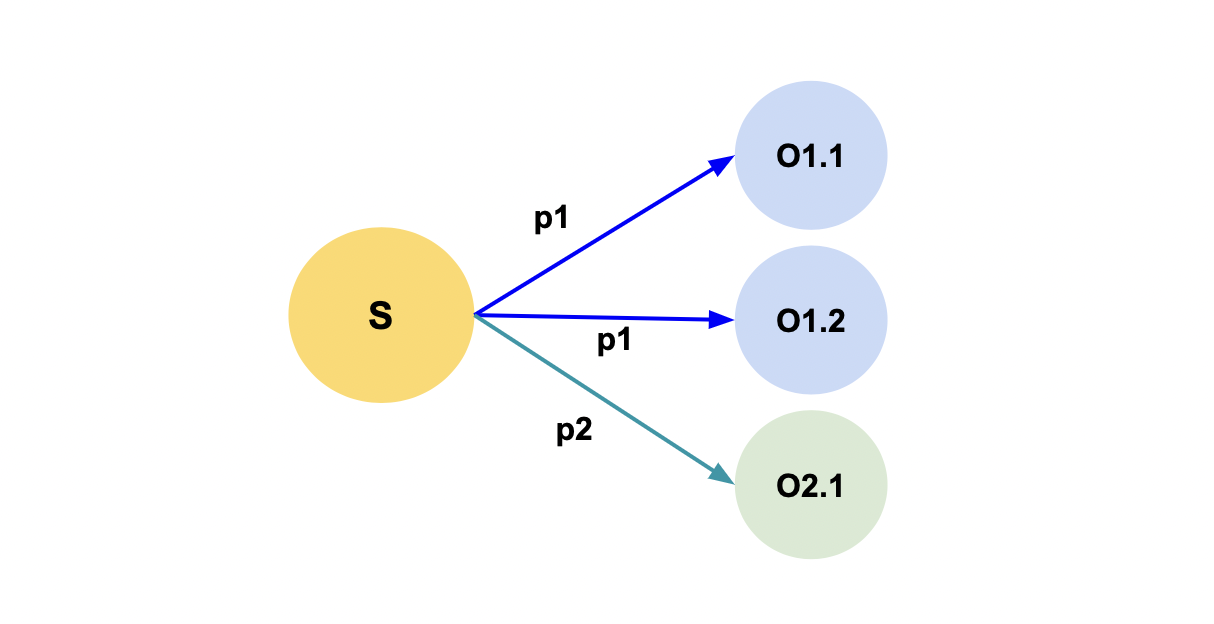
\includegraphics[scale=.3]{Wealth Type 1}
         \caption{Illustration of bag of properties and set of properties}
         \label{fig:wealth-type1}
     \end{subfigure}
     \hfill
     \begin{subfigure}[b]{0.3\textwidth}
         \centering
         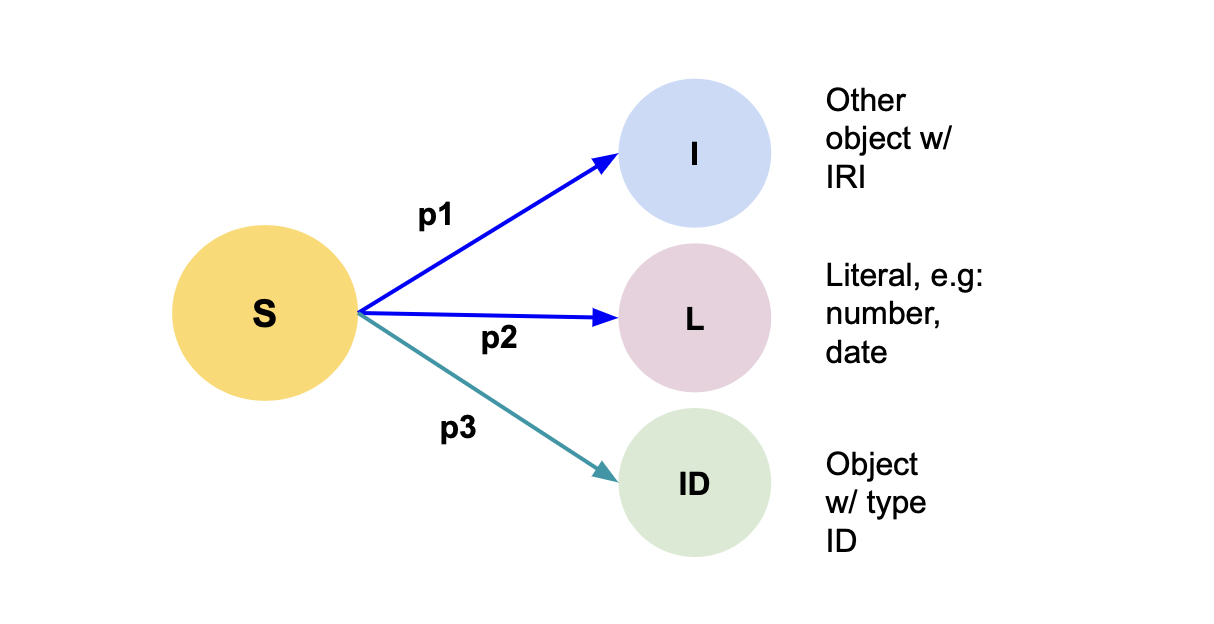
\includegraphics[scale=.3]{Wealth Type 2}
         \caption{Illustration of 3 types of property: object, literal, ID}
         \label{fig:wealth-type2}
     \end{subfigure}
     \hfill
     \begin{subfigure}[b]{0.3\textwidth}
         \centering
         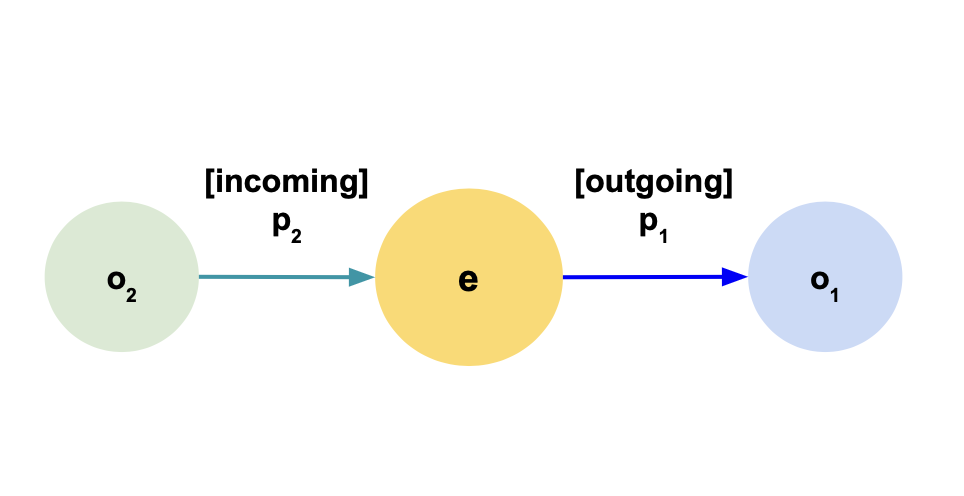
\includegraphics[scale=.3]{Wealth Type 3}
         \caption{Illustration of incoming link vs. outgoing link}
         \label{fig:wealth-type3}
     \end{subfigure}
     \caption{Three simple graphs}
     \label{fig:three graphs}
\end{figure}

Let \(s\) be any entity in a knowledge graph \(G\). We quantify the wealth of entity \(s\) in \(G\) as the amount of information about \(s\) available in \(G\). Thus, the knowledge wealth of an entity is defined by the number of properties associated/linked to it. For example, the wealth of William Shakespeare (Q692) in Wikidata counts all triples describing Q692 in Wikidata, including those detailing his family, occupation, image, and so on.

There are several notion on how to calculate the knowledge wealth of an entity: (1) wealth based on the (non-)uniqueness of individual property; (2) wealth based on type of property; and (3) wealth based on the direction of the link. The wealth of \(s\) with regard to graph \(G\) for each wealth category is denoted by \(W\), formalized and explained as follows.

\paragraph{Wealth based on the (non-)uniqueness of individual properties}
The first measure of the knowledge wealth of \(s\) is bag of properties---the cardinality of set of all triples that has \(s\) in their subject position. In this definition, the triples \((s, p_1, o_1)\) and \((s, p_1, o_2)\) account for a wealth of 1 each, thus both have a total of 2.
Let \(N_{bag}(s,G)\) be a set that comprises all pair of predicate/property and object \((p,o)\) that is connected to \(s\). Then \(W_{bag}(s, G)\) is the cardinality of \(N_{bag}(s,G)\).
\[
    N_{bag}(s,G) = \{(p, o) | (s, p, o) \in G\}
\]
\[
    W_{bag}(s,G) = |N_{bag}(s)|
\]

Another way of measuring the wealth is by counting the number of distinct properties describing the entity, or set of properties. By this way, we are capturing the variety of information about an entity. In contrast to bag of properties, in set of properties \((s, p_1, o_1)\) and \((s, p_1, o_2)\) would be regarded as the "same" information because of the identical property \(p_1\), thus they only account for a total wealth of 1. Let \(N_{set}(s,G)\) be a set that comprises all predicate/property \(p\) that is connected to \(s\). Then \(W_{set}(s, G)\) is the cardinality of \(N_{set}(s,G)\).
\[
    N_{set}(s, G) = \{p | \exists o, (s, p, o) \in G\}
\]
\[
    W_{set}(s, G) = |N_{set}(s,G)|
\]

By the above definition, the wealth of entity \(s\) in \autoref{fig:wealth-type1} is 3 and 2, using bag of properties and set of properties respectively.

\paragraph{Wealth based on type of property}
Object properties are other entities besides \(s\) that is connected with \(s\) through a property \(p\). Wealth of \(s\) using bag of properties with only considering the object properties is defined as:
\[
    W_{bag, object}(s, G) = |\{(p,o) | ((s, p, o) \in G) \cap (o \in I)\}|
\]
Data properties are non-object properties that is connected with \(s\) through a property \(p\). Wealth of \(s\) using bag of properties with only considering the data properties is defined as:
\[
    W_{bag, data}(s, G) = |\{(p,o) | ((s, p, o) \in G) \cap (o \in L)\}|
\]

An external ID is a special type of string that is used to represent an entity in an external source. In Wikidata, an ID is element of subclass of \textit{Wikidata property for an identifier} (Q19847637). Just like any other property, an ID is connected with \(s\) through a property \(p\). Let  \(C_{ID,G}\) be a set comprising ID property in graph \(G\). Wealth of \(s\) using bag of properties with only considering the ID properties is defined as:
\[
    W_{bag, ID}(s, G) = |\{(p,o) | ((s, p, o) \in G) \cap (o \in L) \cap (o \in C_{ID,G})\}|
\]

\paragraph{Wealth based on the direction of the link}
In outgoing link type of wealth, the properties that are used in the wealth calculation of an entity \(s\) are those obtained from link with outwards direction from that particular entity \(s\); that is where \(s\) appears to be the subject in the set of triples in graph \(G\). All types of wealth defined before use the notion of outgoing link.

In incoming link type of wealth, the properties that are used in the wealth calculation of an entity \(s\) are those obtained from link with inwards direction to that particular entity \(s\); that is where \(s\) appears to be the object in the set of triples in graph \(G\). To illustrate, let \(N_{bag}(s)\) be a set that comprises all pair of object and predicate/property \((o,P)\) that is connected to \(s\) in incoming direction to \(s\) i.e., \(N_{bag}(s)\) = \(\{(o, p) | (o, p, s) \in G\}\). Then the wealth of \(s\) using bag of properties and the view of incoming link is notated as \(W_{bag, incoming}(s, G)\), and equal to the cardinality of \(N_{bag}(s)\).
\[
    N_{bag, incoming}(s, G) = \{(o,p) | (o, p, s) \in G\}
\]
\[
    W_{bag, incoming}(s, G) = |N_{bag, incoming}(s, G)|
\]

Looking at in \autoref{fig:wealth-type3}, the wealth of entity \(s\) is 1 using outgoing link, which is from the triple \((s, p_1, o1)\). Its wealth is also 1 and using incoming link, which comes from the triple \((o2, p_2, s)\).

Each definition above can be used simultaneously. For example, the wealth of entity \(s\) using set of properties, calculating object and data but not ID properties, and using the direction of outgoing link is denoted by \(W_{set, outgoing, (object \cup data) \cap ID^\complement}(s, G) = |N_{set, outgoing, (object \cup data) \cap ID^\complement}(s, G)|\) with \(N_{set, outgoing, (object \cup data) \cap ID^\complement}(s, G) = \{p | \exists o, (s, p, o) \in G, \cap (o \in ((I \cup L) \cap C_{ID,G}^\complement)\}\)

\subsubsection{Class-Level Wealth}
Let \(C\) be a class that consists of \(m\) distinct entities \(s_1\), \(s_2\), ... \(s_m\) in graph \(G\). The wealth of \(C\) can be be quantified using its constituent entities. It can be described by several measures, such as entity count, mean and median of its entities' wealth, and percentile of its entities's wealth. To illustrate, let a class \(C\) consists of 4 entities  \(s_1\), \(s_2\), \(s_3\), and \(s_4\) from \autoref{fig:wealth-weighted}. We may say class \(C\) has a total wealth of 4 when we look from count of entities.
\subsection{Insight Model}

\paragraph{Exploratory Data Analysis (EDA): Descriptive Statistics Measures.} Descriptive statistics is concerned with the description and summarization of data. It is a summary of a dataset that helps to describe features of data quantitatively (Ross, 2019). To have a general view of wealth distribution of a class, we use the following measures:
\begin{itemize}
  \item measures of central tendency: mean, median, mode
  \item measures of frequency: count, cumulative frequency/percentage
  \item measures of position: quartile, percentile
  \item measures of dispersion: minimum, maximum, range, interquartile range, standard deviation, coefficient of variation, kurtosis
  \item measures of symmetry: skewness
\end{itemize}


\paragraph{Gini Coefficient}
Gini coefficient is a metric used to measure the economic wealth gaps between countries. A study by Akbar (2020) utilized the Gini coefficient to measure the level of knowledge imbalance in knowledge graphs, particularly Wikidata classes. To calculate the imbalance level of a Wikidata class using Gini coefficient, the researcher started by calculating the number of properties of each entity of that particular class and storing them in an array. The array will then be sorted in descending order, from the smallest to the largest i.e., \(y_{i} \geq y_{i+1} \forall i \in \{1, 2, ..., n\}\). The Gini coefficient will be calculated from the sorted array using the Gini coefficient formula below.

\[G = 1 - \frac{1}{n^{2}\mu} \sum_{i=1}^{n} \sum_{j=1}^{n} Min(y_{i}, y_{j})\]
\[G = 1 + \frac{1}{n} - \frac{1}{n^{2}\mu} - (y_{1} + 2y_{2} + ... + ny_{n})\]

In economics context, \(n\) is the size of population of a country, $\mu$ is the average income, and \(y\) is an array containing data of each country's income. However, in the context of knowledge graph, \(n\) is the number of entities in the class, $\mu$ is the average knowledge wealth of the entities, and \(y\) is an array containing data of each entity's wealth, sorted in descending order.

For example, let's say we have a class that consists of 10 entities. After counting the number of properties of each entities (using the notion of bag of properties for wealth) and sorting them in descending order, we will have an array of \(y = [10,8,8,7,4,2,2,1,1,1]\). The length of the array is \(n = 10\) and the average wealth is \(\mu = 4.4\). Then, apply the Gini coefficient formula and we get \(G = 1 + \frac{1}{10} - \frac{2}{10^{2}\times4.4}(1\times10 + 2\times8 + ... + 10\times1) = 0.414\)

For another another example, let's say we have another array of 10 entities \(z = [10, 9, 9, 9, 9, 9, 9, 9, 9, 5]\). By applying the same formula to z, we get a Gini coefficient value of \(0.052\).

The Gini coefficient has a value between \(0\) and \(1\). The higher the coefficient value, the greater the imbalance level. The value of 0 is achieved when all observed entities have the same amount of wealth. The value of 1 occurs when all income is owned solely by one entity and this phenomenon expresses full inequality.


\paragraph{Lorenz Curve} Lorenz curve is a graphical representation of wealth inequality (The Lorenz Curve: What It Tells You About Economic Inequality, 2022). It shows how the wealth is cumulatively distributed, with data points sorted from the poorest to the richest. \textit{(Here, give the example of Lorenz Curve)}. In Lorenz curve, the horizontal axis represents the fraction of the population, and the vertical axis represents the cumulative wealth. Therefore, if the point (\textit{x}, \textit{y}) = (30, 15) lies on the curve, then we can interpret that the bottom 30\% of the population account for 15\% of the total wealth in that population. The Lorenz curve is usually drawn along with a straight diagonal line with a slope of 1. This straight line represents perfect equality in wealth distribution, i.e., each individual in the observed population has equal wealth. The Lorenz curve itself is drawn below the straight line. The ratio of the area between the Lorenz curve and the straight line of perfect equality to the triangular area below the straight line, is the Gini coefficient.

\subsection{Sample Application of Formal and Insight Model}

\begin{figure}[!htbp]
    \centering
    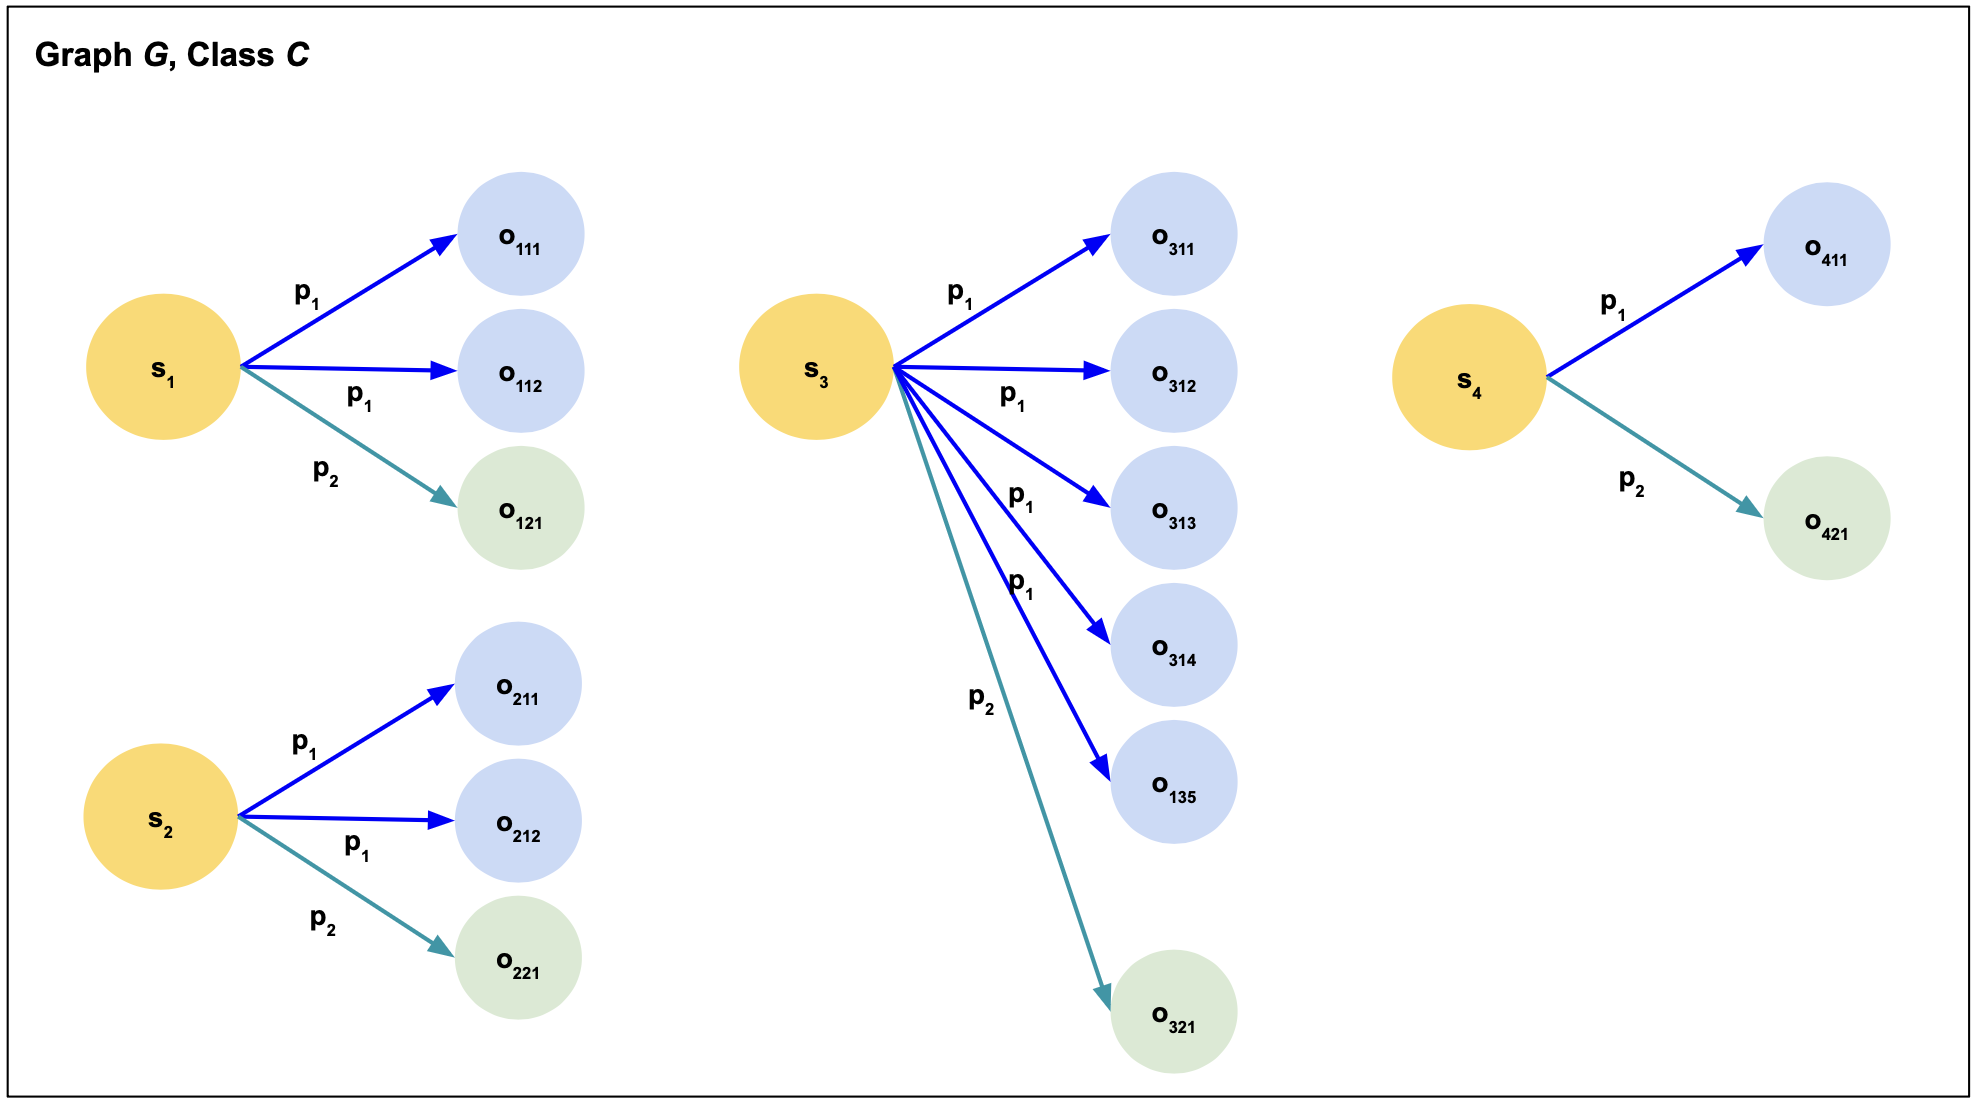
\includegraphics[scale=.4]{Wealth Weighted}
    \caption{Sample knowledge graph \(G\) that contains class \(C\) with 4 entities} \label{fig:wealth-weighted}
\end{figure}

We provide small case in \autoref{fig:wealth-weighted} to illustrate how both models can be applied in quantifying knowledge wealth. In this example, we will focus on the notion using bag of properties with outgoing direction of link to quantify the wealth.

A graph \(G\) has a class \(C\), which consists of four entities \(s_1\), \(s_2\), \(s_3\), and \(s_4\). Each entity has two distinct properties \(p_1\) and \(p_2\). For example, entity \(s_1\) is linked by property \(p_1\) to objects \(o_{111}\) and \(o_{112}\), and by property \(p_2\) to object \(o_{121}\). Using the bag of properties and outgoing link direction, the wealth of entity \(s_1\) is 3 (2 accounted for by \(p_1\) and 1 by \(p_2\)). Similarly, the wealth of entities \(s_2\), \(s_3\), and \(s_4\) is 3, 6, and 2, respectively. \autoref{tab:sample statistical summary} provides a statistical summary describing the wealth of class \(C\). Entities in class \(C\) have a mean wealth of 3.5, a median wealth of 3, a mode wealth of 3, a minimum wealth of 2, and a maximum wealth of 6. Based on each individual entity's wealth, the imbalance measure of class \(C\) is quantified using the Gini coefficient, which has a value of 0.21.

\begin{center}
    \small
    \begin{threeparttable}
    \caption{Statistical Summary of Wealth of Class \(C\)}
    \label{tab:sample statistical summary}
    \begin{tabular}{c | c c c c c c c} 
    
    \toprule
        Measure & Entity Count & Mean & Median & Mode & Minimum & Maximum & Gini \\ [0.5ex] 
    \midrule
        Value & 4 & 3.5 & 3 & 3 & 2 & 6 & 0.21 \\
        [0.5ex]
    \bottomrule
    \end{tabular}
    \begin{tablenotes}
        \footnotesize
        \item{This table shows some statistical measures to quantify the wealth of class \(C\).}
    \end{tablenotes}
    \end{threeparttable}
\end{center}

In addition to the Gini coefficient, the Lorenz curve for the wealth of entities in class \(C\) is shown in \autoref{fig:sample-lorenz}. This figure illustrates that the wealth distribution within class \(C\) is very close to the diagonal line of perfect equality, which aligns with the small Gini coefficient value of 0.21.

\begin{figure}[!htbp]
    \centering
    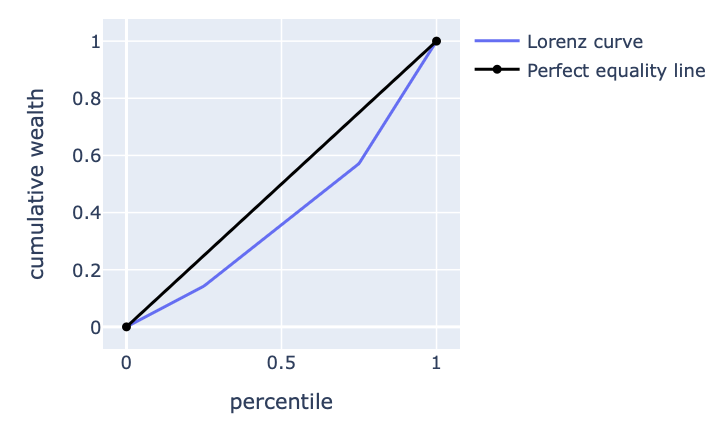
\includegraphics[scale=0.8]{Sample Lorenz Curve}
    \caption{Lorenz curve of class \(C\)} \label{fig:sample-lorenz}
\end{figure}
\subsection{Python-Based Model Implementation}

Our study provides a Python-based implementation library for both the formal model and the insight model. The library incorporates the three notions of knowledge wealth discussed in \autoref{wealth-formal-model}, as well as the insight model outlined in \autoref{insight-model}. While the model is platform-agnostic, i.e., it can be applied to any KG, we focus its implementation on Wikidata for demonstrating its use cases. Wikidata is specifically chosen because of the availability of Wikidata Query Service which  facilitates structured queries over its data.

The notions of wealth are implemented at the query level, meaning that the filters and aggregations based on each wealth definition are directly embedded in SPARQL queries. The flow begins with defining class filters to specify the entities of interest. Next, SPARQL querying is performed using Wikidata Query Service to retrieve RDF triples matching the specified criteria and aggregate them according to the selected notion of wealth. The extracted data is then structured into pandas DataFrames, enabling further analysis through the insight model using Python libraries.

In our implementation, we only consider direct properties and exclude blank nodes to reduce complexity and maintain data quality. The complete flow of the formal model and insight model usage is illustrated in \autoref{fig:model-implementation}.

\begin{figure}[!htbp]
    \centering
    % 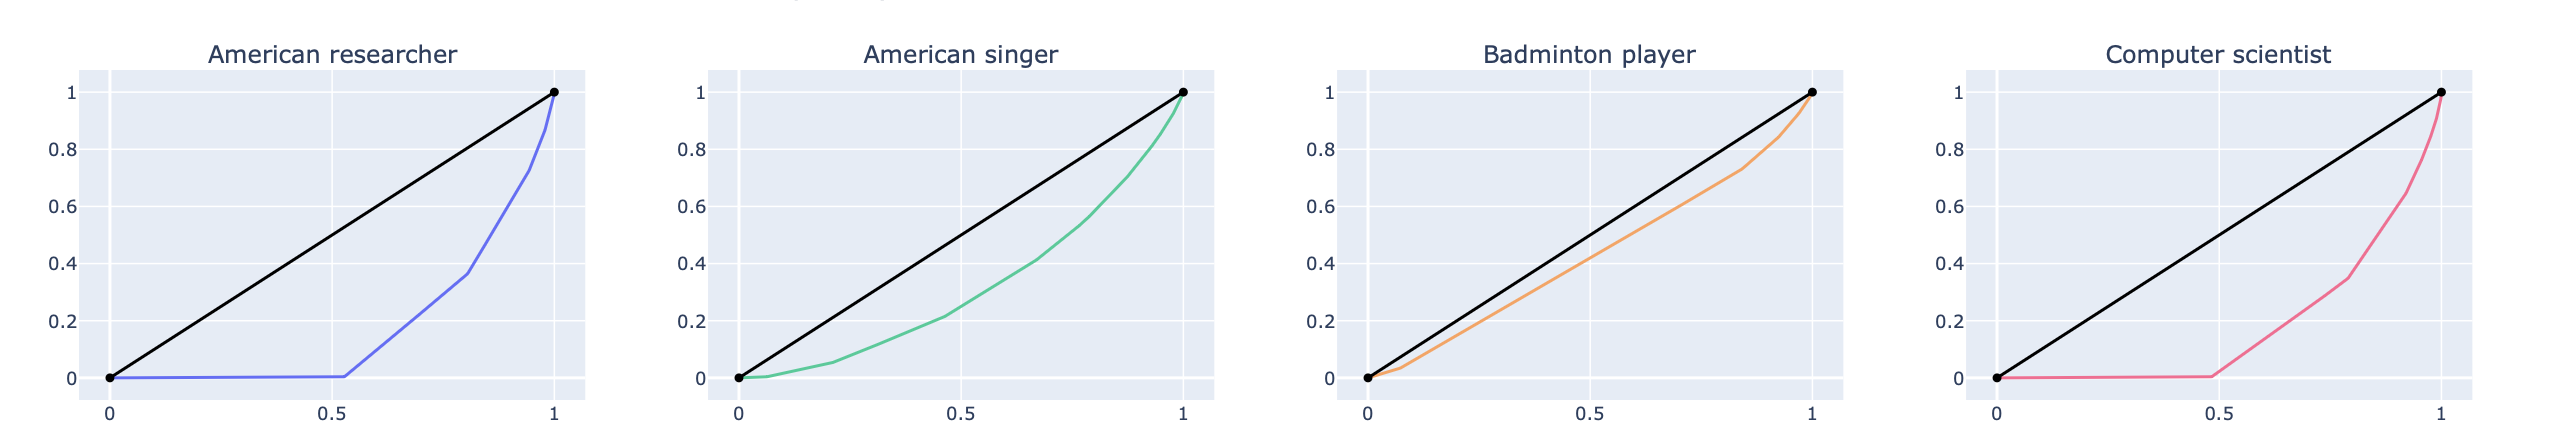
\includegraphics[scale=.5]{Gini - Pure Literal}
    \makebox[\textwidth][c]{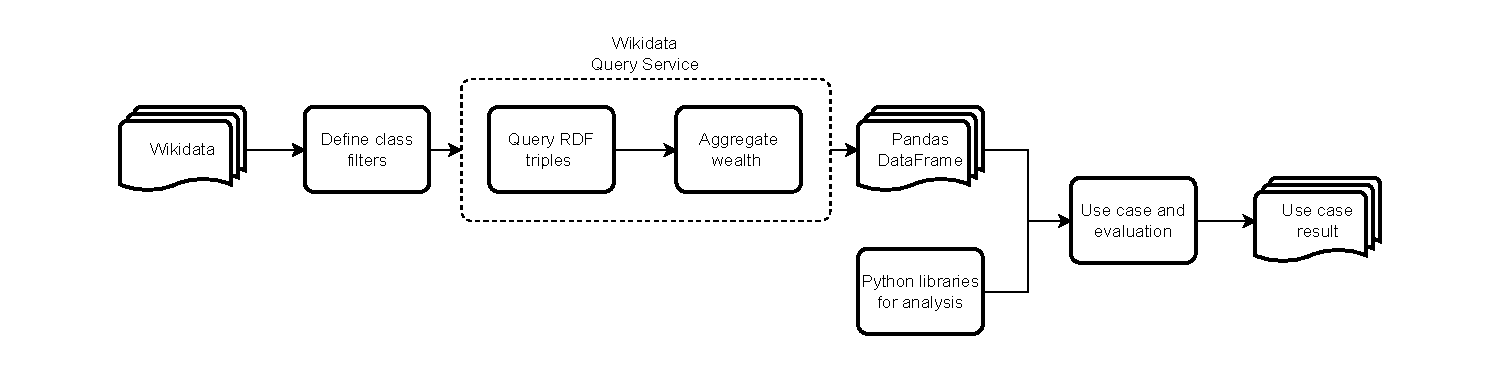
\includegraphics[width=1\textwidth]{Model Implementation.pdf}}%
    \caption{Model implementation and evaluation flow using Python Jupyter Notebook} \label{fig:model-implementation}
\end{figure}